\chapter{Binary Solid--Liquid Diagrams}\label{ch:b2:solid-liquid-diagrams}

Tin melts at \qty{232}{\degreeCelsius} and lead at \qty{327}{\degreeCelsius},
yet the old solder of electricians, a mixture of the two, melts at
\qty{182}{\degreeCelsius}, below both. Salt spread on a road melts ice, but only
down to about \qty{-21}{\degreeCelsius}; on a colder night it does nothing.
Copper and nickel, on the other hand, mix in any proportion even in the
solid, and their alloys melt over a range of temperatures between those of the
two metals. The diagrams of this chapter tell, for each pair, which solids
crystallise from a cooling liquid, at which temperatures and in which
amounts --- the knowledge behind every casting, every solder joint and every
low-melting alloy.

\begin{recall}
\Cref{ch:b2:chemical-potential}: \omterm{def:b2:chemical-potential:chemical-potential}{chemical potential} of a component in an \omterm{def:b2:chemical-potential:ideal-mixture}{ideal
mixture}, cryoscopy. \Cref{ch:b2:equilibrium-shifts}: the \omterm{def:b2:equilibrium-shifts:variance}{variance}.
\Cref{ch:b2:liquid-vapour-diagrams}: \omterm{def:b2:liquid-vapour-diagrams:binary-diagram}{binary diagrams}, tie lines and the \omterm{thm:b2:liquid-vapour-diagrams:lever}{lever
rule}. The Year 1 volume: metallic bonding, substitutional and interstitial
alloys, crystal types.
\end{recall}

\begin{omfigure}
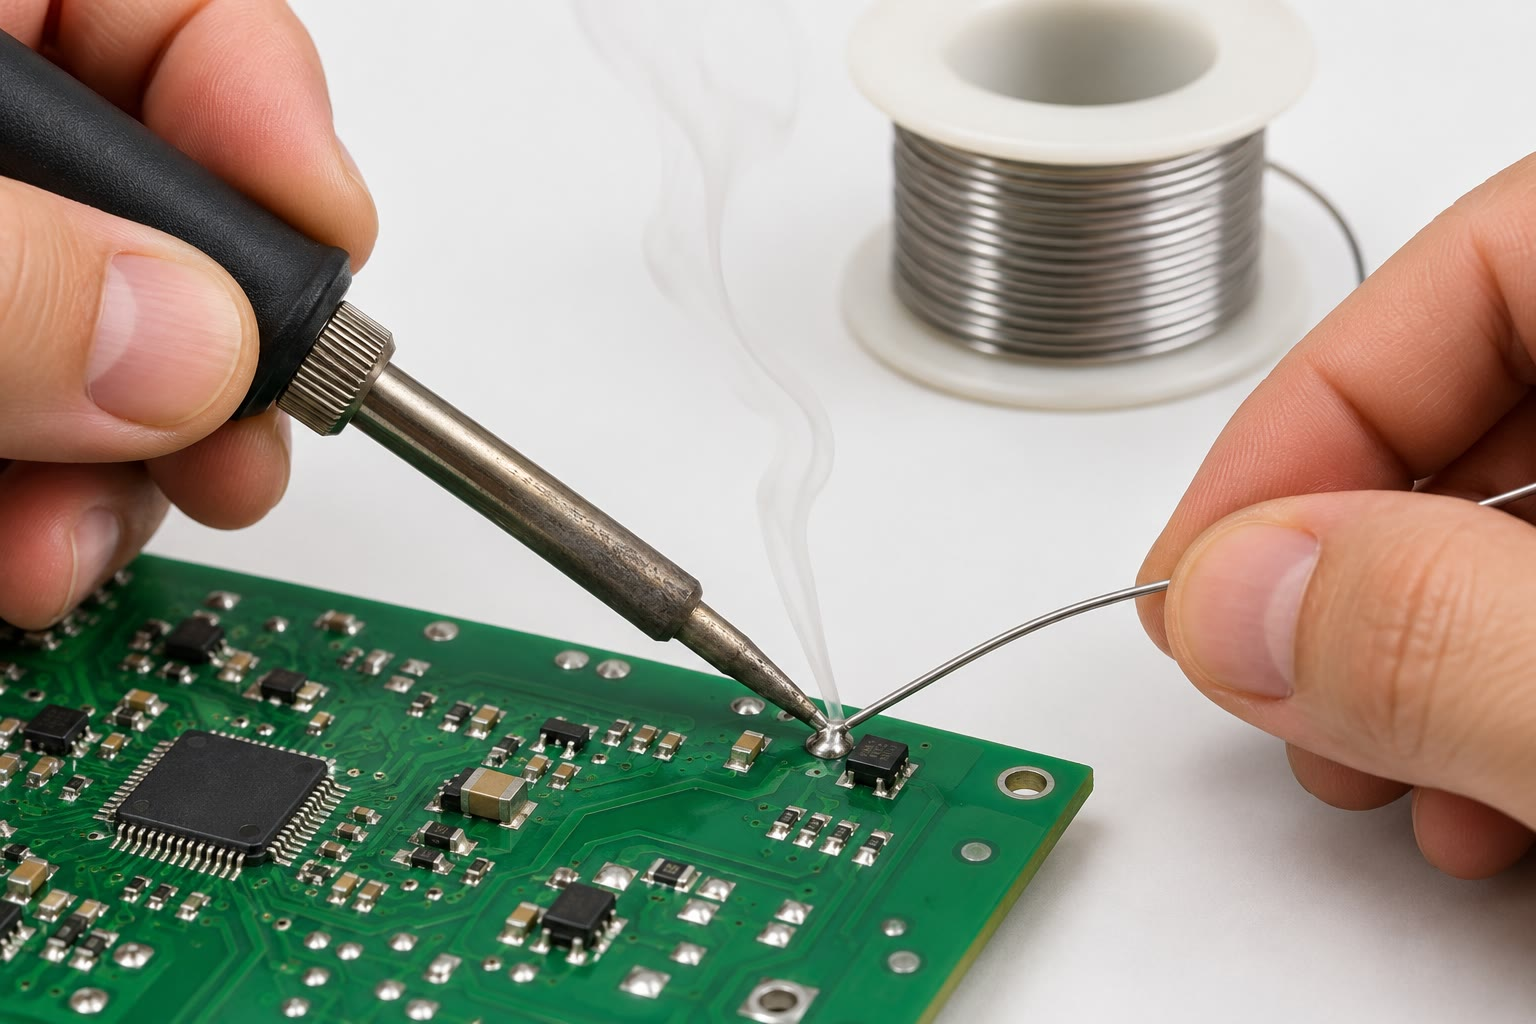
\includegraphics[width=0.6\linewidth]{images/book3/ai/b2-08-soldering.jpg}

{\small Soldering a component on a circuit board: the wire of solder melts on
contact with the hot iron and the joint freezes within a second when the iron
is lifted --- because the alloy melts at a single, low temperature.}
\end{omfigure}

\section{Thermal analysis}

\begin{definition}[Thermal analysis]\label{def:b2:solid-liquid-diagrams:cooling-curve}
\emph{Thermal analysis}\index{thermal analysis} determines the temperatures of
the changes of state of a sample from its temperature recorded while it is
heated or cooled at a steady rate. The record of temperature against time
during a slow cooling is a \emph{cooling curve}\index{cooling curve}.
\end{definition}

Far from any change of state, the sample cools smoothly. When a solid starts to
crystallise, the heat of crystallisation slows the cooling: the curve shows a
break in slope, or stops at a constant temperature for a while --- a
\textit{plateau} --- if the freezing occurs at fixed temperature.

\begin{proposition}[Plateaus]\label{prop:b2:solid-liquid-diagrams:plateaus}
At fixed pressure, a pure substance freezes at constant temperature, and so
does a binary liquid from which two solids crystallise together. A binary
liquid from which one solid crystallises freezes over a range of temperatures.
\end{proposition}

\begin{proof}
With the pressure fixed, the \omterm{def:b2:equilibrium-shifts:variance}{variance} is $v = n - r + 1 - \varphi$. Pure
substance, liquid + solid: $v = 1 + 1 - 2 = 0$. Binary, liquid + two solids:
$v = 2 + 1 - 3 = 0$. Binary, liquid + one solid: $v = 2 + 1 - 2 = 1$: the
temperature changes as the liquid composition does. A \omterm{def:b2:equilibrium-shifts:variance}{variance} 0 means the
temperature cannot change while all the phases are present: the heat removed is
supplied by the freezing, until a phase disappears.
\end{proof}

\begin{omfigure}
\begin{tikzpicture}[font=\small, x=0.55cm, y=0.05cm]
  \foreach \dx/\name in {0/pure metal, 9/{mixture, one solid first}, 18/eutectic mixture} {
    \draw[->] (\dx,0) -- (\dx+7.5,0) node[below left, font=\scriptsize] {$t$};
    \draw[->] (\dx,0) -- (\dx,62) node[above, font=\scriptsize] {$T$};
    \node[font=\scriptsize] at (\dx+3.8,-8) {\name};
  }
  % pure: cool, plateau at 40, cool
  \draw[omDef, thick] (0,58) .. controls (1,48) and (1.6,42) .. (2,40) -- (4.5,40) .. controls (5.2,32) and (6,24) .. (7,20);
  \node[font=\scriptsize, anchor=south] at (3.25,40.5) {plateau};
  % mixture: cool, break at 48, slow fall, plateau at 30, cool
  \draw[omDef, thick] (9,58) .. controls (9.6,53) and (9.9,50) .. (10.2,48)
     .. controls (11,42) and (11.6,35) .. (12.3,30) -- (14.2,30) .. controls (14.9,23) and (15.6,17) .. (16.5,14);
  \node[font=\scriptsize, anchor=west] at (10.4,49.5) {break};
  \node[font=\scriptsize, anchor=south] at (13.25,30.5) {eutectic};
  % eutectic: plateau at 30
  \draw[omDef, thick] (18,58) .. controls (19,46) and (19.8,36) .. (20.5,30) -- (24,30) .. controls (24.7,23) and (25.4,17) .. (26.2,14);
  \node[font=\scriptsize, anchor=south] at (22.25,30.5) {plateau};
\end{tikzpicture}

{\small \omterm{def:b2:solid-liquid-diagrams:cooling-curve}{Cooling curves}, schematic. A pure metal freezes on a plateau. A
mixture shows a break in slope when the first solid appears, then the slow
cooling of a liquid that freezes over a range of temperatures, then the
plateau of the eutectic. A liquid of the eutectic composition freezes on a
single plateau, like a pure substance.}
\end{omfigure}

\begin{method}[Building a diagram from cooling curves]\label{met:b2:solid-liquid-diagrams:diagram-from-curves}
\begin{enumerate}
  \item Record \omterm{def:b2:solid-liquid-diagrams:cooling-curve}{cooling curves} for a series of compositions, pure components
        included.
  \item On a (composition, temperature) graph, plot for each composition the
        temperature of the first break (the start of crystallisation) and of
        each plateau.
  \item Join the points of first crystallisation: this is the \omterm{def:b2:solid-liquid-diagrams:liquidus}{liquidus}. Join
        the ends of freezing: the \omterm{def:b2:solid-liquid-diagrams:liquidus}{solidus}. A plateau found at the same
        temperature for many compositions is an invariant line (a eutectic).
  \item The length of the eutectic plateau, largest at the eutectic
        composition, locates that composition.
\end{enumerate}
\end{method}

\section{Total miscibility in the solid}

\begin{definition}[Solid solution]\label{def:b2:solid-liquid-diagrams:solid-solution}
A \emph{solid solution}\index{solid solution} is a single crystalline phase of
variable composition, in which atoms of one component replace atoms of the
other on the sites of the same lattice (substitutional) or occupy the holes of
that lattice (interstitial).
\end{definition}

Copper and nickel have the same face-centred cubic structure and atoms of close
radii: they form a substitutional \omterm{def:b2:solid-liquid-diagrams:solid-solution}{solid solution} at every composition.

\begin{definition}[Liquidus and solidus]\label{def:b2:solid-liquid-diagrams:liquidus}
On a solid--liquid diagram the \emph{liquidus}\index{liquidus} is the curve
above which everything is liquid; it gives the composition of the liquid in
equilibrium with a solid. The \emph{solidus}\index{solidus} is the curve below
which everything is solid; where the solid is a solution, it gives the
composition of the solid in equilibrium with the liquid.
\end{definition}

\begin{proposition}[The lens]\label{prop:b2:solid-liquid-diagrams:lens}
If the two components form ideal solutions in the liquid and in the solid,
the \omterm{def:b2:solid-liquid-diagrams:liquidus}{liquidus} and the \omterm{def:b2:solid-liquid-diagrams:liquidus}{solidus} join the two melting points and enclose a
lens-shaped two-phase domain; at each temperature the mole fraction $x_i$ of
each component in the liquid and in the solid are related by
\[
  \frac{x_i^{\ell}}{x_i^{s}} = \exp\left[-\frac{\Delta_{\text{fus}}H_i}{R}\left(\frac1T - \frac1{T_i^*}\right)\right] .
\]
\end{proposition}

\begin{proof}
The \omterm{def:b2:chemical-potential:chemical-potential}{chemical potential} of $i$ is the same in both phases, $\mu_i^{*,s} +
RT\ln x_i^s = \mu_i^{*,\ell} + RT\ln x_i^\ell$, so $RT\ln(x_i^\ell/x_i^s) =
-(\mu_i^{*,\ell} - \mu_i^{*,s}) = -\Delta_{\text{fus}}G_i(T)$, and with constant
$\Delta_{\text{fus}}H_i$, $\Delta_{\text{fus}}G_i = \Delta_{\text{fus}}H_i(1 - T/T_i^*)$.
Together with $x_1 + x_2 = 1$ in each phase, the two relations fix the two
compositions at each $T$ (solved numerically for the figure); that the
resulting curves form a lens is admitted.
\end{proof}

\begin{omfigure}
\begin{tikzpicture}
\begin{axis}[omphase, width=0.62\linewidth, height=7cm, ymin=1050, ymax=1480,
  xlabel={$x$ (nickel)}, ylabel={$T$ (\unit{\degreeCelsius})}]
\addplot[omliquidus] table[x=xl, y=T] {figdata/out/bachelor-2-solid-liquid-a.dat};
\addplot[omsolidus] table[x=xs, y=T] {figdata/out/bachelor-2-solid-liquid-a.dat};
\draw[tieline] (axis cs:0.541,1300) -- (axis cs:0.609,1300);
\fill (axis cs:0.58,1300) circle (1.3pt);
\node[font=\scriptsize] at (axis cs:0.25,1400) {liquid};
\node[font=\scriptsize] at (axis cs:0.8,1150) {solid solution};
\node[font=\scriptsize, anchor=east] at (axis cs:0.5,1330) {liquidus};
\node[font=\scriptsize, anchor=west] at (axis cs:0.66,1290) {solidus};
\node[font=\scriptsize, anchor=west] at (axis cs:0.03,1080) {\qty{1085}{\degreeCelsius}};
\draw[black!50] (axis cs:0.005,1084) -- (axis cs:0.03,1080);
\node[font=\scriptsize, anchor=south east] at (axis cs:1.0,1456) {\qty{1455}{\degreeCelsius}};
\end{axis}
\end{tikzpicture}

{\small Copper--nickel, computed for ideal solid and liquid solutions from the
melting points and enthalpies of fusion of the two metals. At
\qty{1300}{\degreeCelsius} an alloy of composition 0.58 is split into a liquid
of 0.541 and a solid of 0.609 (dashed tie line).}
% ledger: tfus:Cu, dfus:Cu, tfus:Ni, dfus:Ni
\end{omfigure}

\begin{method}[Reading a solid--liquid diagram]\label{met:b2:solid-liquid-diagrams:read-solid-liquid}
\begin{enumerate}
  \item Follow the vertical line of the overall composition downwards from the
        liquid.
  \item On the \omterm{def:b2:solid-liquid-diagrams:liquidus}{liquidus}, the first solid appears; its composition is read on
        the other end of the tie line (the \omterm{def:b2:solid-liquid-diagrams:liquidus}{solidus}, or a pure component).
  \item In the two-phase domain, read the two compositions at the ends of the
        tie line and the proportions by the \omterm{thm:b2:liquid-vapour-diagrams:lever}{lever rule}, in moles with mole
        fractions, in mass with mass fractions.
  \item On a horizontal invariant line, the temperature stops until one phase
        has gone; below it, read the new pair of phases.
\end{enumerate}
\end{method}

\begin{example}[An alloy at \qty{1300}{\degreeCelsius}]\label{ex:b2:solid-liquid-diagrams:lever}
For the alloy of nickel mole fraction 0.58 at \qty{1300}{\degreeCelsius}, the
fraction of the atoms in the solid is $(0.58 - 0.541)/(0.609 - 0.541) = 0.57$.
The first solid to appear, near \qty{1315}{\degreeCelsius}, is richer in nickel
than the alloy, the last liquid poorer.
\end{example}

The diagram describes equilibrium, which in a solid is slow: the first crystals,
rich in nickel, are covered by layers poorer and poorer in it as the liquid
changes, and diffusion in the solid has no time to even them out. A casting
cooled quickly is made of \textit{cored} crystals, graded from the centre to the
edge; a long heating below the \omterm{def:b2:solid-liquid-diagrams:liquidus}{solidus} homogenises them.

\section{No miscibility in the solid: the eutectic}

When the two solids do not mix at all, each component crystallises pure, and
the \omterm{def:b2:solid-liquid-diagrams:liquidus}{liquidus} has two branches, one per solid.

\begin{theorem}[Schr\"oder--van Laar]\label{thm:b2:solid-liquid-diagrams:schroder}
If a component A crystallises pure from an ideal liquid mixture, the \omterm{def:b2:solid-liquid-diagrams:liquidus}{liquidus}
on which the solid A appears is given by
\[
  \ln x_A = -\frac{\Delta_{\text{fus}}H_A}{R}\Big(\frac1T - \frac1{T_A^*}\Big),
\]
with $x_A$ the mole fraction of A in the liquid, $T_A^*$ and
$\Delta_{\text{fus}}H_A$ the melting point and enthalpy of fusion of pure A
(taken as constant).
\end{theorem}

\begin{proof}
At equilibrium, the \omterm{def:b2:chemical-potential:chemical-potential}{chemical potential} of pure solid A equals that of A in the
liquid: $\mu_A^{*,s}(T) = \mu_A^{*,\ell}(T) + RT\ln x_A$. Hence $R\ln x_A =
-\Delta_{\text{fus}}G_A(T)/T$. By Gibbs--Helmholtz, $d(\Delta_{\text{fus}}G_A/T)/
dT = -\Delta_{\text{fus}}H_A/T^2$; integrating from $T_A^*$, where
$\Delta_{\text{fus}}G_A = 0$, to $T$ gives $\Delta_{\text{fus}}G_A/T =
\Delta_{\text{fus}}H_A(1/T - 1/T_A^*)$.
\end{proof}

For a dilute solution, $\ln x_A = \ln(1 - x_B) \approx -x_B$ and $1/T -
1/T_A^* \approx -\Delta T/T_A^{*2}$: $\Delta T = RT_A^{*2}x_B/\Delta_{\text{fus}}H_A$,
the cryoscopic law of \cref{ch:b2:chemical-potential}. For benzene ($T^* =
\qty{278.64}{K}$, $\Delta_{\text{fus}}H = \qty{9.87}{kJ/mol}$, $M =
\qty{78.11}{g/mol}$), the \omterm{def:b2:chemical-potential:colligative}{cryoscopic constant} $RT^{*2}M/\Delta_{\text{fus}}H$
comes out as \qty{5.11}{K.kg/mol}.
% ledger: tfus:benzene, dfus:benzene

\begin{definition}[Eutectic]\label{def:b2:solid-liquid-diagrams:eutectic}
The \emph{eutectic point}\index{eutectic point} of a binary system is the
point where the liquid is in equilibrium with two solids at once; it is the
lowest temperature at which a liquid exists in that part of the diagram. A
liquid of the eutectic composition, and the fine intimate mixture of the two
solids into which it freezes, are called a \emph{eutectic
mixture}\index{eutectic mixture}.
\end{definition}

\begin{corollary}[The eutectic is where the liquidus branches meet]\label{cor:b2:solid-liquid-diagrams:eutectic}
For two components immiscible in the solid and ideal in the liquid, the
eutectic temperature $T_E$ and composition are the solution of
$x_A(T_E) + x_B(T_E) = 1$, each $x$ given by the Schr\"oder--van Laar equation
of its own solid.
\end{corollary}

\begin{proof}
At the eutectic the liquid is saturated with both solids: it lies on both
branches at once, with the same composition read in A and in B.
\end{proof}

\begin{omfigure}
\begin{tikzpicture}
\begin{axis}[omphase, width=0.62\linewidth, height=6.5cm, ymin=-25, ymax=85,
  xlabel={$x$ (naphthalene)}, ylabel={$T$ (\unit{\degreeCelsius})}]
\addplot[omliquidus] table[x=x, y=T] {figdata/out/bachelor-2-solid-liquid-b-benzene.dat};
\addplot[omliquidus] table[x=x, y=T] {figdata/out/bachelor-2-solid-liquid-b-naphthalene.dat};
\draw[thick] (axis cs:0,-3.55) -- (axis cs:1,-3.55);
\fill (axis cs:0.133,-3.55) circle (1.5pt);
\node[font=\scriptsize, anchor=north] at (axis cs:0.133,-4.5) {E};
\node[font=\scriptsize] at (axis cs:0.45,72) {liquid};
\node[font=\scriptsize, align=center] at (axis cs:0.65,22) {liquid + solid\\ naphthalene};
\node[font=\scriptsize, anchor=south west] at (axis cs:0.08,45) {liquid + solid benzene};
\draw[thin] (axis cs:0.12,45) -- (axis cs:0.06,0.8);
\node[font=\scriptsize] at (axis cs:0.55,-15) {solid benzene + solid naphthalene};
\end{axis}
\end{tikzpicture}

{\small Benzene--naphthalene, computed with the Schr\"oder--van Laar
equation for each solid. The two branches meet at the eutectic E,
\qty{-3.5}{\degreeCelsius} and 0.13 naphthalene, below which all is solid.}
% ledger: tfus:benzene, dfus:benzene, tfus:naphthalene, dfus:naphthalene
\end{omfigure}

\begin{example}[Cooling a benzene--naphthalene mixture]\label{ex:b2:solid-liquid-diagrams:naphthalene}
A liquid of naphthalene mole fraction 0.5 cools until the naphthalene branch
of the \omterm{def:b2:solid-liquid-diagrams:liquidus}{liquidus}, near \qty{46}{\degreeCelsius}, where pure solid naphthalene
starts to crystallise. The liquid, losing naphthalene, slides down the
branch; at \qty{-3.5}{\degreeCelsius} it reaches the eutectic, and the rest
freezes at constant temperature into the \omterm{def:b2:solid-liquid-diagrams:eutectic}{eutectic mixture}. By the \omterm{thm:b2:liquid-vapour-diagrams:lever}{lever rule},
just above the eutectic, the solid naphthalene is $(0.5 - 0.133)/(1 - 0.133) =
42~\%$ of the moles, the eutectic liquid 58~\%.
\end{example}

\begin{proposition}[Length of the eutectic plateau]\label{prop:b2:solid-liquid-diagrams:plateau-length}
For samples of the same mass cooled with the same rate of heat removal, the
duration of the eutectic plateau is proportional to the amount of liquid that
reaches the eutectic, maximal for the eutectic composition and zero for the
pure components.
\end{proposition}

\begin{proof}
On the plateau the temperature is constant: the heat removed, $\Phi\,\Delta t$
at a constant rate $\Phi$, is the heat released by the freezing of the
eutectic liquid, $m_E\,\Delta_{\text{fus}}h_E$. So $\Delta t = m_E\,\Delta_{\text{fus}}h_E/
\Phi$, proportional to the mass $m_E$ of eutectic liquid, which the \omterm{thm:b2:liquid-vapour-diagrams:lever}{lever
rule} gives.
\end{proof}

\section{Partial miscibility and defined compounds}

Most pairs of metals are neither fully miscible nor fully immiscible in the
solid: each dissolves a little of the other. Lead dissolves up to 19~\% of tin
by mass, tin up to 3.4~\% of lead. The diagram then holds two \omterm{def:b2:solid-liquid-diagrams:solid-solution}{solid
solutions}, (Pb) and (Sn), and a eutectic between them; the eutectic line no
longer reaches the sides of the diagram, but stops at the limits of the \omterm{def:b2:solid-liquid-diagrams:solid-solution}{solid
solutions}.

\begin{omfigure}
\begin{tikzpicture}[font=\small, x=0.075cm, y=0.022cm]
  \draw[->] (0,0) -- (106,0) node[right] {\% Sn (mass)};
  \draw[->] (0,0) -- (0,360) node[above] {$T$ (\unit{\degreeCelsius})};
  \foreach \t in {100,200,300} \draw (0,\t) -- (-1.5,\t) node[left, font=\scriptsize] {\t};
  \foreach \w in {0,20,40,60,80,100} \draw (\w,0) -- (\w,-5) node[below, font=\scriptsize] {\w};
  % invariant points (NIST): Pb 327.5, Sn 231.9, eutectic 182.2 at 62.13; limits 18.91 and 96.59
  \draw[omliquidus] (0,327.5) .. controls (25,290) and (45,235) .. (62.13,182.2);
  \draw[omliquidus] (100,231.9) .. controls (85,215) and (72,200) .. (62.13,182.2);
  \draw[omsolidus] (0,327.5) .. controls (8,280) and (14,220) .. (18.91,182.2);
  \draw[omsolidus] (100,231.9) .. controls (98.5,215) and (97.5,200) .. (96.59,182.2);
  \draw[thick] (18.91,182.2) -- (96.59,182.2);
  \draw[omsolidus, densely dashed] (18.91,182.2) .. controls (12,120) and (6,60) .. (3,20);
  \draw[omsolidus, densely dashed] (96.59,182.2) .. controls (98.5,120) and (99.3,60) .. (99.6,20);
  \fill (62.13,182.2) circle (1.5pt);
  \fill (18.91,182.2) circle (1.2pt); \fill (96.59,182.2) circle (1.2pt);
  \node[anchor=south, font=\scriptsize] at (62.13,186) {E};
  \node[font=\scriptsize] at (55,300) {liquid};
  \node[font=\scriptsize] at (6,150) {(Pb)};
  \node[font=\scriptsize] at (103,140) {(Sn)};
  \node[font=\scriptsize] at (28,235) {L + (Pb)};
  \node[font=\scriptsize] at (84,192) {L + (Sn)};
  \node[font=\scriptsize] at (55,100) {(Pb) + (Sn)};
  % cooling path at 40 %
  \draw[->, omProp, thick] (40,340) -- (40,30);
  \node[font=\scriptsize, omProp, anchor=south] at (40,342) {40~\%};
  \node[font=\scriptsize, anchor=north east] at (16.6,179) {18.9};
  \node[font=\scriptsize, anchor=north] at (62.13,178) {62.1};
  \node[font=\scriptsize, anchor=north east] at (95.8,178) {96.6};
  \node[font=\scriptsize, anchor=west] at (101,182.2) {\qty{182.2}{\degreeCelsius}};
\end{tikzpicture}

{\small The lead--tin diagram, drawn through its invariant points: melting
points of lead (\qty{327.5}{\degreeCelsius}) and tin (\qty{231.9}{\degreeCelsius}),
eutectic E at \qty{182.2}{\degreeCelsius} and 62.1~\% tin, limits of the \omterm{def:b2:solid-liquid-diagrams:solid-solution}{solid
solutions} at the eutectic temperature (18.9~\% and 96.6~\% tin). The curves
between those points, and the dashed solubility limits below the eutectic,
are drawn schematically. Arrow: the cooling of a 40~\% solder.}
% ledger: eut:Pb-Sn.T, eut:Pb-Sn.wL, eut:Pb-Sn.wPb, eut:Pb-Sn.wSn, tfus:Pb, tfus:Sn
\end{omfigure}

A 40~\% tin solder starts to freeze on the \omterm{def:b2:solid-liquid-diagrams:liquidus}{liquidus} by depositing crystals of
the lead-rich solution (Pb); the liquid grows richer in tin until, at
\qty{182.2}{\degreeCelsius}, it reaches the eutectic composition and freezes into
a fine mixture of (Pb) and (Sn) lamellae, around the primary crystals.

\begin{omfigure}
\begin{tikzpicture}[font=\small]
  \begin{scope}
    \clip (0,0) circle (2.2);
    \fill[gray!20] (-2.3,-2.3) rectangle (2.3,2.3);
    \foreach \k in {-24,...,24} \draw[gray!65, line width=1.1pt] (-2.4+0.2*\k,-2.4) -- ++(55:6);
    \foreach \cx/\cy/\r/\a in {-0.9/0.8/0.55/10, 0.7/1.0/0.45/40, 0.2/-0.6/0.6/-20, -1.1/-0.9/0.4/70, 1.3/-0.3/0.35/5} {
      \fill[omDef!35, draw=omDef, rotate around={\a:(\cx,\cy)}] (\cx,\cy) ellipse ({\r} and {0.7*\r});
    }
  \end{scope}
  \draw[thick] (0,0) circle (2.2);
  \draw[<-, omProp, thick] (0.7,1.0) -- (3.0,1.6) node[right, text=black] {primary (Pb) crystal};
  \draw[<-, omProp, thick] (1.6,0.9) -- (3.0,0.5) node[right, text=black, align=left] {eutectic: alternate\\ (Pb) and (Sn) lamellae};
\end{tikzpicture}

{\small The microstructure of a 40~\% tin solder after slow cooling, schematic:
primary crystals of (Pb), formed between the \omterm{def:b2:solid-liquid-diagrams:liquidus}{liquidus} and the eutectic, in a
matrix of eutectic made of thin alternating plates of the two \omterm{def:b2:solid-liquid-diagrams:solid-solution}{solid
solutions}.}
\end{omfigure}

\begin{definition}[Defined compound]\label{def:b2:solid-liquid-diagrams:defined-compound}
A \emph{defined compound}\index{defined compound} is a solid of fixed
composition $\mathrm{A}_a\mathrm{B}_b$ formed by the two components. It shows
\emph{congruent melting}\index{congruent melting} when it melts into a liquid of
its own composition: the \omterm{def:b2:solid-liquid-diagrams:liquidus}{liquidus} then has a maximum at that composition.
\end{definition}

A compound with \omterm{def:b2:solid-liquid-diagrams:defined-compound}{congruent melting} splits the diagram in two: each half, A with
$\mathrm{A}_a\mathrm{B}_b$ and $\mathrm{A}_a\mathrm{B}_b$ with B, is a diagram of
its own, with its own eutectic. The composition of the maximum, read in mole
fraction, gives the formula of the compound.

\begin{omfigure}
\begin{tikzpicture}[font=\small, x=6cm, y=0.05cm]
  \draw[->] (0,0) -- (1.06,0) node[right] {$x_{\mathrm B}$};
  \draw[->] (0,0) -- (0,95) node[above] {$T$};
  \node[below, font=\scriptsize] at (0,0) {A}; \node[below, font=\scriptsize] at (1,0) {B};
  \node[below, font=\scriptsize] at (0.667,0) {$\tfrac23$};
  \draw[omliquidus] (0,70) .. controls (0.12,58) and (0.25,45) .. (0.35,35);
  \draw[omliquidus] (0.35,35) .. controls (0.45,62) and (0.58,79) .. (0.667,80);
  \draw[omliquidus] (0.667,80) .. controls (0.75,79) and (0.8,68) .. (0.85,50);
  \draw[omliquidus] (0.85,50) .. controls (0.9,56) and (0.95,62) .. (1,65);
  \draw[thick] (0,35) -- (0.667,35); \draw[thick] (0.667,50) -- (1,50);
  \draw[thick] (0.667,0) -- (0.667,80);
  \fill (0.35,35) circle[radius=1.5pt]; \fill (0.85,50) circle[radius=1.5pt];
  \fill (0.667,80) circle[radius=1.5pt];
  \node[anchor=north, font=\scriptsize] at (0.35,34) {E$_1$};
  \node[anchor=north, font=\scriptsize] at (0.85,49) {E$_2$};
  \node[anchor=south, font=\scriptsize] at (0.667,81) {$\mathrm{AB_2}$ melts};
  \node[font=\scriptsize] at (0.35,80) {liquid};
  \node[font=\scriptsize, align=center] at (0.33,15) {A +\\ $\mathrm{AB_2}$};
  \node[font=\scriptsize, align=center] at (0.84,25) {$\mathrm{AB_2}$\\ + B};
\end{tikzpicture}

{\small Schematic diagram with a \omterm{def:b2:solid-liquid-diagrams:defined-compound}{defined compound} $\mathrm{AB_2}$ (vertical
line at $x_{\mathrm B} = 2/3$) melting congruently at the maximum of the
\omterm{def:b2:solid-liquid-diagrams:liquidus}{liquidus}. The diagram is two simple eutectic diagrams side by side, with
eutectics E$_1$ and E$_2$.}
\end{omfigure}

\section{Uses}

\paragraph{Solders and low-melting alloys.} A solder must melt below the parts
it joins and freeze quickly, without a pasty range: the eutectic composition is
the natural choice. The tin--lead eutectic melts at \qty{182.2}{\degreeCelsius};
because lead is toxic, electronics now use lead-free solders, among them the
bismuth--tin eutectic, which melts at \qty{138.8}{\degreeCelsius} and contains
57~\% bismuth by mass.
% ledger: eut:Pb-Sn.T, eut:Bi-Sn.T, eut:Bi-Sn.wL

\paragraph{De-icing.} Ice and salt form a eutectic: the ice--salt dihydrate
eutectic lies at \qty{252}{K} (\qty{-21}{\degreeCelsius}) and 23.3~\% sodium
chloride by mass. Above that temperature, salt in contact with ice forms a
brine whose freezing point is below the temperature of the road, and the ice
melts; below it, no liquid can exist, and salt is useless.
% ledger: eut:NaCl-water.T, eut:NaCl-water.w

\paragraph{Crystallisation.} The diagram of a salt and water is read like any
other: cooling a hot saturated solution crosses the solubility curve (the
\omterm{def:b2:solid-liquid-diagrams:liquidus}{liquidus} of the salt), and pure crystals of the salt are deposited while the
impurities, too dilute to reach their own \omterm{def:b2:solid-liquid-diagrams:liquidus}{liquidus}, stay in the mother liquor.
This is the purification by recrystallisation of the Year 1 volume, seen on a
diagram.

\begin{omfigure}
\begin{tikzpicture}
\begin{axis}[omphase, width=0.62\linewidth, height=6cm, xmin=0, xmax=100,
  ymin=90, ymax=285, xlabel={\% Bi (mass)}, ylabel={$T$ (\unit{\degreeCelsius})}]
\addplot[omliquidus] table[x=w, y=T] {figdata/out/bachelor-2-solid-liquid-d-Sn.dat};
\addplot[omliquidus] table[x=w, y=T] {figdata/out/bachelor-2-solid-liquid-d-Bi.dat};
\draw[densely dashed] (axis cs:0,119.5) -- (axis cs:100,119.5);
\fill[omThm] (axis cs:56.97,138.8) circle (2pt);
\node[font=\scriptsize, omThm, anchor=west] at (axis cs:64,129) {assessed eutectic};
\draw[omThm, thin] (axis cs:64,129) -- (axis cs:57.8,137.6);
\node[font=\scriptsize, anchor=north] at (axis cs:52,118) {ideal model};
\node[font=\scriptsize] at (axis cs:50,250) {liquid};
\end{axis}
\end{tikzpicture}

{\small Bismuth--tin: the \omterm{def:b2:solid-liquid-diagrams:liquidus}{liquidus} predicted for pure solids and an ideal
liquid (Schr\"oder--van Laar, blue) meets at a eutectic near
\qty{120}{\degreeCelsius}; the assessed eutectic (red dot) lies at
\qty{138.8}{\degreeCelsius} and 57~\% bismuth.}
% ledger: tfus:Sn, dfus:Sn, tfus:Bi, dfus:Bi, eut:Bi-Sn.T, eut:Bi-Sn.wL
\end{omfigure}

\section{Exercises}

\begin{exercise}[$\star$]\label{exo:b2:solid-liquid-diagrams:1}
On the copper--nickel diagram, give the phases present at
\qty{1300}{\degreeCelsius} for nickel mole fractions 0.40, 0.58 and 0.70.
\end{exercise}

\begin{exercise}[$\star$]\label{exo:b2:solid-liquid-diagrams:2}
\qty{2.00}{mol} of a copper--nickel alloy of nickel mole fraction 0.58 are held
at \qty{1300}{\degreeCelsius}. Compute the amounts of solid and liquid and the
amount of nickel in each.
\end{exercise}

\begin{exercise}[$\star$]\label{exo:b2:solid-liquid-diagrams:3}
Compute the \omterm{def:b2:equilibrium-shifts:variance}{variance} at fixed pressure (a) of a pure metal while it freezes;
(b) of a copper--nickel alloy while it freezes; (c) of a lead--tin liquid on the
eutectic line.
\end{exercise}

\begin{exercise}[$\star$]\label{exo:b2:solid-liquid-diagrams:4}
Sketch the \omterm{def:b2:solid-liquid-diagrams:cooling-curve}{cooling curve} of pure tin from \qty{300}{\degreeCelsius} to
\qty{100}{\degreeCelsius} and explain why the temperature stops at
\qty{232}{\degreeCelsius}.
\end{exercise}

\begin{exercise}[$\star\star$]\label{exo:b2:solid-liquid-diagrams:5}
With the data of the chapter (benzene \qty{278.64}{K}, \qty{9.87}{kJ/mol};
naphthalene \qty{353.2}{K}, \qty{19.1}{kJ/mol}), check that at
\qty{269.6}{K} the two Schr\"oder--van Laar mole fractions add up to 1, and give
the eutectic composition.
\end{exercise}

\begin{exercise}[$\star\star$]\label{exo:b2:solid-liquid-diagrams:6}
Describe the cooling of a lead--tin alloy of 30~\% tin by mass, from the liquid
to room temperature, and compute the mass fraction of eutectic it contains.
\end{exercise}

\begin{exercise}[$\star\star$]\label{exo:b2:solid-liquid-diagrams:7}
What mass of sodium chloride per kilogram of water does the eutectic brine
contain? Why is salting a road useless at \qty{-25}{\degreeCelsius}?
\end{exercise}

\begin{exercise}[$\star\star$]\label{exo:b2:solid-liquid-diagrams:8}
On the schematic diagram with the compound $\mathrm{AB_2}$, describe the
cooling of liquids of $x_{\mathrm B} = 0.5$ and $x_{\mathrm B} = 0.9$: first
solid, eutectic reached, solids at the end.
\end{exercise}

\begin{exercise}[$\star\star$]\label{exo:b2:solid-liquid-diagrams:9}
In zone refining, a molten zone is passed slowly along a bar. Near pure nickel,
the ratio of the copper mole fractions in the solid and in the liquid at
equilibrium is about 0.78. Explain why the copper is carried along with the
molten zone, and why several passes are needed.
\end{exercise}

\begin{exercise}[$\star\star\star$]\label{exo:b2:solid-liquid-diagrams:10}
Derive the Schr\"oder--van Laar equation, then show that for a dilute liquid
it reduces to $\Delta T = K_f\,b$, with $K_f = RT^{*2}M_A/\Delta_{\text{fus}}H_A$
and $b$ the molality of the solute; compute $K_f$ for benzene.
\end{exercise}

\begin{exercise}[$\star\star\star$]\label{exo:b2:solid-liquid-diagrams:11}
The magnesium--lead diagram has a \omterm{def:b2:solid-liquid-diagrams:liquidus}{liquidus} maximum at 19.0~\% magnesium by
mass. Find the formula of the compound.
\end{exercise}

\begin{exercise}[$\star\star\star$]\label{exo:b2:solid-liquid-diagrams:12}
Equal masses of lead--tin alloys are cooled under the same conditions. The
eutectic alloy shows a plateau of \qty{300}{s}; an unknown alloy shows one of
\qty{120}{s}. Find the two possible compositions of the unknown, and say how to
tell them apart.
\end{exercise}

\section{Problem: Solder}

\begin{problem}[{Weekend problem --- the lead--tin diagram from its invariant
points, the freezing of a 40~\% solder by the lever rule, a lead-free
bismuth--tin solder predicted by the ideal-liquid model, and the choice of a
solder}]
\label{pb:b2:solid-liquid-diagrams:1}
Data (NIST, calculated invariant equilibria): lead--tin eutectic at
\qty{182.2}{\degreeCelsius}, liquid of 62.13~\% tin by mass, in equilibrium with
(Pb) of 18.91~\% and (Sn) of 96.59~\% tin; bismuth--tin eutectic at
\qty{138.8}{\degreeCelsius}, liquid of 56.97~\% bismuth. Melting points and
enthalpies of fusion: lead \qty{600.6}{K}, \qty{4.77}{kJ/mol}; tin
\qty{505.1}{K}, \qty{7.03}{kJ/mol}; bismuth \qty{544.6}{K}, \qty{11.30}{kJ/mol}.
Molar masses (\unit{g/mol}): Pb 207.2, Sn 118.71, Bi 208.98.
% ledger: eut:Pb-Sn.T, eut:Pb-Sn.wL, eut:Pb-Sn.wPb, eut:Pb-Sn.wSn, eut:Bi-Sn.T, eut:Bi-Sn.wL, tfus:Pb, dfus:Pb, tfus:Sn, dfus:Sn, tfus:Bi, dfus:Bi, aw:Pb, aw:Sn, aw:Bi

\medskip
\noindent\textbf{Part I --- The lead--tin diagram.}
\begin{enumerate}
  \item Convert the melting points of lead and tin to degrees Celsius.
  \item Convert the eutectic composition to a mole fraction of tin.
  \item Place on a (mass \% Sn, $T$) graph the melting points, the eutectic and
        the two ends of the eutectic line.
  \item Draw the diagram and name its six domains.
  \item Write the eutectic transformation on cooling.
  \item Compute the \omterm{def:b2:equilibrium-shifts:variance}{variance} on the eutectic line at fixed pressure.
\end{enumerate}

\medskip
\noindent\textbf{Part II --- Cooling a 40~\% solder.}
\begin{enumerate}[resume]
  \item Which solid appears first, and why is it not pure lead?
  \item How does the composition of the liquid change during the cooling down
        to the eutectic?
  \item Just above \qty{182.2}{\degreeCelsius}: which phases, of which
        compositions?
  \item Compute their mass fractions.
  \item Just below: which phases, of which compositions, and in which mass
        fractions?
  \item What fraction of the alloy is made of eutectic constituent, and what
        fraction of primary (Pb) crystals?
  \item Sketch the \omterm{def:b2:solid-liquid-diagrams:cooling-curve}{cooling curve} and compare its plateau with that of the
        eutectic alloy.
\end{enumerate}

\medskip
\noindent\textbf{Part III --- A lead-free solder by the ideal-liquid model.}
\begin{enumerate}[resume]
  \item Write the Schr\"oder--van Laar equation for the \omterm{def:b2:solid-liquid-diagrams:liquidus}{liquidus} of tin.
  \item Write it for the \omterm{def:b2:solid-liquid-diagrams:liquidus}{liquidus} of bismuth.
  \item Write the condition defining the eutectic.
  \item Compute the sum of the two mole fractions at \qty{110}{\degreeCelsius},
        \qty{120}{\degreeCelsius} and \qty{130}{\degreeCelsius}, and find the
        eutectic temperature of the model to the nearest degree.
  \item Give the eutectic composition of the model, in mole and in mass
        fraction of bismuth.
  \item Compare with the assessed eutectic.
  \item Tin dissolves up to 21~\% of bismuth in the solid. Explain how this
        makes the real eutectic hotter than the model's.
\end{enumerate}

\medskip
\noindent\textbf{Part IV --- Choosing a solder.}
\begin{enumerate}[resume]
  \item Why is a eutectic composition preferred for a solder?
  \item Give one reason to replace lead in solders.
  \item What does the low melting point of the bismuth--tin eutectic offer, and
        what could it cost?
  \item Compute the masses of bismuth and tin in \qty{1.00}{kg} of
        bismuth--tin eutectic solder.
  \item State the eutectic temperature of bismuth--tin predicted by the
        ideal-liquid model.
\end{enumerate}
\end{problem}
